\chapter{Non-linear methods}{The world does not behave linearly. Models do.} \label{cahpNonLinear}
The previous chapters introduce regression and classification, presenting numerical example from linear models. Often, linear models cannot be applied in practice since they simplify too much the behaviour of reality. For this reason, non-linear models are implemented to build supervised models both for regression, and classification. Well-established mathematical models define non-linear models. Differently from linear models that the solving approach is not exact, but approximated by efficient heuristics.\par

This chapter presents non-linear models according to the classification of machine learning methods into the five tribes ~\cite{Domingos2015}. Each tribe is related to a specific branch of science whose researchers are used to learn and make discoveries with a precise technique. Each tribe has a precise way of working:

\begin{enumerate}
    \item Evolutionaries create knowledge by evolving structures;
    \item Connectionists create knowledge by learning parameters;
    \item Symbolists create knowledge by composing element on the fly;
    \item Bayesians create knowledge by weighting evidence;
    \item Analogisers create knowledge by mapping to new situations.
\end{enumerate}

All these tribes have a precise way of thinking, a specific optimisation algorithm, an evaluation metric and a representation tool (i.e. the formal language of each tribe). Figure \ref{fig_tribes}, introduced in ~\cite{Domingos2015} illustrates all these elements and suppose the existence of a master algorithm able to merge the five approaches, aiming at learning anything.

% INSERT fig_tribes
\begin{figure}[hbt!]
\centering
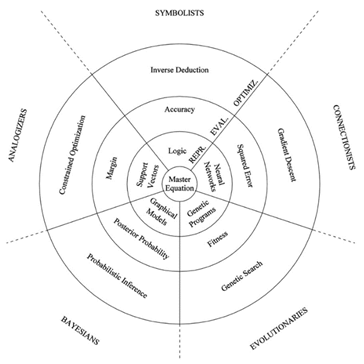
\includegraphics[width=0.9\textwidth]{SectionLetsMath/nonLinearMethods_fig/fig_tribes.png}
\captionsetup{type=figure}
\caption{The five tribes optimisation, evaluation, and representation tools.}
\label{fig_tribes}
\end{figure}


\section{Evolutionaries’ methods}

The name evolutionaries comes from the theory of evolution of Charles Darwin ~\cite{Darwin1859}. With this tribe, we refer to researchers and methods born in the field of biology to model and understand how nature evolves. The machine learning tribe called evolutionaries mimics the natural behaviour to learn information.\par

The formal language of evolutionaries is the genetic programming and thinking that leads to classification systems, as the classification of the species. Their evaluation metric is the goodness of fit that measures the distance between the outcome of a model and its true value. Evolutionaries use search algorithms that move on the input data hyperplane to find solutions. These algorithms are called genetic search algorithms and belong to the family of metaheuristics.

\subsection{Genetic search} \label{geneticSearch}
Genetic search algorithms are metaheuristic algorithms that consider an initial feasible solution of a prescriptive problem and make it evolve by mimics of the natural evolution mechanisms as mutations and cross-over. They aim at finding a new feasible solution with a better performing solution value. \par

Figure \ref{fig_mutation} identifies the mutation of a string of data, where a bit of the original input has been randomly changed. The impact of this mutation on the solution value is evaluated by the goodness of fit of the model.

% INSERT fig_mutation
\begin{figure}[hbt!]
\centering
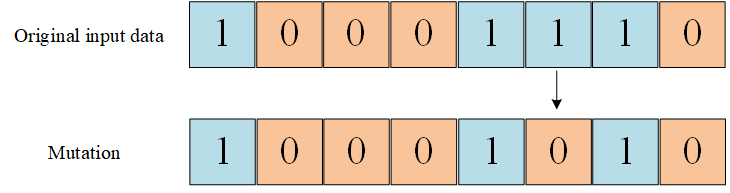
\includegraphics[width=0.9\textwidth]{SectionLetsMath/nonLinearMethods_fig/fig_mutation.png}
\captionsetup{type=figure}
\caption{Example of mutation of a string of data.}
\label{fig_mutation}
\end{figure}

Figure \ref{fig_crossover} identifies an example of a cross-over of two strings of data. The values of the string are pivoted around a splitting point and combined to generate two new strings. The fitness function evaluates if the cross-over leads to an improvement of the solution value.


% INSERT fig_crossover
\begin{figure}[hbt!]
\centering
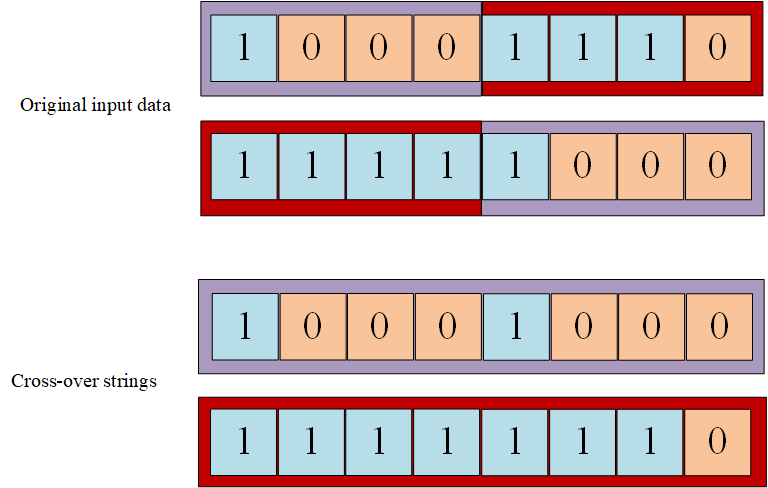
\includegraphics[width=0.9\textwidth]{SectionLetsMath/nonLinearMethods_fig/fig_crossover.png}
\captionsetup{type=figure}
\caption{Example of cross-over of a string of data.}
\label{fig_crossover}
\end{figure}


\section{Symbolists’ methods} 

The symbolists use the formal language of the logic to learn and generate information. We already introduced the logic in \ref{chapLogicalModelling}, and we have already seen the application of logic to unsupervised learning models in the definition of association rules (see Section \ref{secAssociationRules}). A similar “if-else” statement can be used to learn information in a supervised fashion by using decision trees. Decision trees are the application of the formal language of symbolists to supervised learning. Their evaluation metric is measured through the accuracy and the information gain.\footnote{The package logproj provides methods to deal with symbolists' methods \href{https://github.com/aletuf93/logproj/blob/master/logproj/M_learningMethod/symbolists_models.py}{here}.}

\subsection{Decision trees} \label{secDecisionTrees}
Decision trees can be used both for regression and for classification. The idea behind a regression tree is to split the space of the input features into $M$ partitions such that the response of the model is:

\begin{equation}
        f\left(x\right)=\sum_{m=1}^{M}{c_mI\left(x\in R_m\right)}
        \label{eq_decisionTree1}
\end{equation}

In other words, the model assigns a constant response value $c_m$ for each partition $m$ of the feature space. The model can be represented as a tree where the observations are split based on the value of a splitting variable $j$ and a splitting point $s$. Each branch, consequently, divide the current feature region into two regions $R_1$ and $R_2$ such that $R_1\left(j,s\right)=\{X|X_j\le s\}$ and  $R_2\left(j,s\right)=\{X|X_j>s\}$.The branching variable $j$ and its splitting point $s$ are chosen to minimize the error function:

\begin{equation}
        \min_{j,s}{\left[\min_{c_1}{\sum_{x_i\in R_1(j,s)}\left(y_i-c_1\right)^2}+\min_{c_2}{\sum_{x_i\in R_2(j,s)}\left(y_i-c_2\right)^2}\right]}
        \label{eq_decisionTree2}
\end{equation}

At each stage of the tree, all the splitting points $s$ are tested for each variable $j$ very quickly defining two new partitions of the feature space. The responses $c_1$ and $c_2$ are defined as:

\begin{equation}
\begin{split}
        c_1=E[(y_i|x_i\in R_1\left(j,s\right))]\\
        c_2=E[{(y}_i|x_i\in R_2\left(j,s\right))]\\
\end{split}
\label{eq_decisionTree3}
\end{equation}

A minimum node size can be predetermined to avoid an exponential growth of the number of nodes of the tree. Alternatively, a tree node can be split only if the decrease in the sum-of-squares exceeds a threshold. This can be expressed using a cost-complexity criterion:

\begin{equation}
        C_\alpha\left(T\right)=\sum_{m=1}^{\left|T\right|}{N_mQ_m\left(T\right)+\alpha\left|T\right|}
        \label{eq_decisionTree4}
\end{equation}

Where $N_m=card(x_i\in R_m)$, $c_m=\frac{1}{N_m}\sum_{x_i\in R_m} y_i$ and $Q_m\left(T\right)=\frac{1}{N_m}\sum_{x_i\in R_m}\left(y_i-c_m\right)^2$. $Q_m\left(T\right)$ is a measure of impurity in each partitioned region, the equation (\ref{eq_decisionTree4}) aim at defining a subtree that controls the tradeoff between impurity and the growth of the tree.\par

Classification trees work as regression trees with a different definition of the impurity function. Classification trees offer different impurity functions $Q_m(T)$:
\begin{itemize}
    \item The misclassification error $Q_m(T)\ =\ 1-p_{mk}$;
    \item The Gini index $Q_m(T)\ =\ \sum_{k=1}^{K}{p_{mk}(1-p_{mk})}$;
    \item The cross-entropy $Q_m(T)\ =\ -\sum_{k=1}^{K}{p_{mk}\log{p_{mk}}}$.
\end{itemize}

All these impurity functions are based on the value of $p_{mk}$, i.e. the proportion of class $k$ observation in node $m$.

\begin{equation}
        p_{mk}=\frac{1}{N_m}\sum_{x_i\in R_m}{I(y_i=k)}
        \label{eq_decisionTree5}
\end{equation}
Where $N_m=card(x_i\in R_m)$.\par 

Similarly to regression trees, a new branch of a decision tree is opened if it reduces the value of the impurity function at that node $m$ compared to the weighted impurity of the nodes of the new sub-tree.\par

When implementing a decision tree, it is possible to measure the relative importance of an input feature $l$ by using:
\begin{equation}
        I_l^2\left(T\right)=\sum_{t=1}^{J-1}{{\hat{i}}_t^2I\left(v\left(t\right)=l\right)}
        \label{eq_decisionTree6}
\end{equation}
Where $J-1$ are the internal nodes of the regression tree $T$ and ${\hat{i}}_t^2$ is the maximal estimated improvement in the squared error risk obtained by choosing $l$ as splitting variable at the node $t$. 

\section{Bayesians’ methods} \label{secBayesianMethods}

Bayesian methods rely on the well known Bayes' theorem that we already introduced in section \ref{secBayesTheorem}. By using prior and posterior probability, we have the possibility to update the belief we have on an event when new observation (e.g. new data or data from another data source) are available. The formal language of the bayesians is the graphical modelling as Bayesian and Markov networks. The posterior probability given from the empirical observation is the evaluation metric of these models. The search method is the averaging between initial beliefs given by the prior (i.e. the initial assumptions) and the posterior (i.e. the empirical evidence).\footnote{The package logproj provides methods to deal with bayesians' methods \href{https://github.com/aletuf93/logproj/blob/master/logproj/M_learningMethod/bayesians_models.py}{here}.}

\subsection{Naïve Bayes}
The prior probability of the Bayes theorem reflects the initial belief we have on an event. The posterior probability indicates all the other data we add to support or discard our initial belief. When applying the Bayes theorem to machine learning, we obtain a relationship between causes (i.e. the input dataset $X$) and effect (the target variable $y$):

\begin{equation}
        P\left(cause\middle| effect\right)=\frac{P\left(cause\right)\times P(effect|cause)}{P(effect)}
        \label{eq_naiveBayes1}
\end{equation}
Unluckily, phenomena have many causes leading to and effect. \par

We have already seen that any machine learning model can be interpreted as a method to estimate the joint probability distribution between the input features, and the target (i.e. the cause, and the effects). Naïve Bayes approaches this problem simply, by assuming all the causes, i.e. the input features are independent. Under this assumption, the joint density distribution is obtained as:

\begin{equation}
        f_j\left(X\right)=\prod_{k=1}^{p}{f_{jk}(X_k)}
        \label{eq_naiveBayes2}
\end{equation}

Each marginal density distribution can be estimated using one-dimensional kernel density estimation (see section \ref{secKernelDensityEstimation}). Naïve Bayes calculates the product of these kernels, and the logit transform is, then, used to get a model in an additive form (similar to the perceptron algorithm illustrated in chapter \ref{chapLinearClassification}).

\begin{equation}
\begin{split}
        \log\left(\frac{Prob\{G=l|X\}}{Prob\{G=J|X\}}\right) & =\log\left(\frac{\pi_lf_l(X)}{\pi_Jf_J(X)}\right)=\\
        & =\log{\left(\frac{\pi_l\prod_{k=1}^{P}{f_{lk}(X_k)}}{\pi_J\prod_{k=1}^{P}{f_{Jk}(X_k)}}\right)=}\\
        & =\log{\left(\frac{\pi_l}{\pi_J}\right)+\sum_{k=1}^{P}\log{\left(\frac{f_{lk}(X_k)}{f_{Jk}(X_k)}\right)=}}\\
        & =\alpha_l+\sum_{k=1}^{P}{g_{lk}(X_k)}
\end{split}
\label{eq_naiveBayes3}
\end{equation}

\subsection{Markov Chain} \label{secMarkovChain}
The hypothesis of the independence between the input variables is hardly often valid. On the other side, the definition of an accurate joint probability distribution requires a huge amount of data and a significant computational time. To overcome these obstacles, Markov chains assume that the probability of an event only depends on the current state of a system. \par

The p attributes of the input dataset $X$ define the state of a system, and they are linked together by a transition probability. This way, even if the number of features $p$ is high, the number of transition probabilities $t$ calculate is still limited. Figure \ref{fig_markovChain} introduce the graphical model of a Markov chain, whose information content is described by a transition matrix $T$ with states $i$ and $j$ as rows and columns labels. The entries $t_{ij}\in T$ identifies the probabilities from $i$ to $j$.

% INSERT fig_markovChain
\begin{figure}[hbt!]
\centering
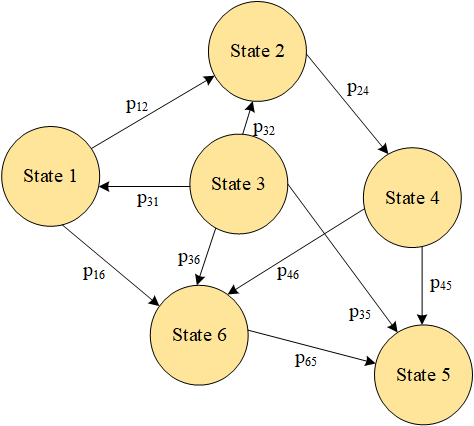
\includegraphics[width=0.7\textwidth]{SectionLetsMath/nonLinearMethods_fig/fig_markovChain.png}
\captionsetup{type=figure}
\caption{Network of a Markov chain.}
\label{fig_markovChain}
\end{figure}

\subsection{Hidden Markov Model and Kalman filter} \label{secKalmanFilter}
Sometimes, state variables are not observable, but the state depends on a subset of measurable variables that affect the state variables, and a model (i.e. a prior) of how these variables affect the state is given (see Figure \ref{fig_hiddenMarkovModel}).

% INSERT fig_hiddenMarkovModel
\begin{figure}[hbt!]
\centering
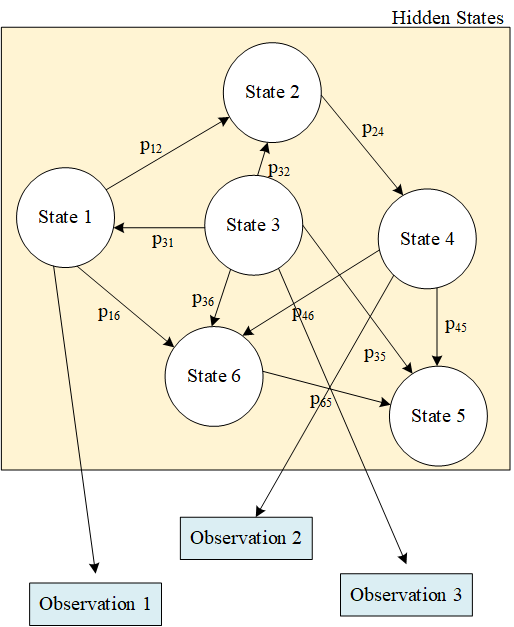
\includegraphics[width=0.7\textwidth]{SectionLetsMath/nonLinearMethods_fig/fig_hiddenMarkovModel.png}
\captionsetup{type=figure}
\caption{Network of a Hidden Markov Model}
\label{fig_hiddenMarkovModel}
\end{figure}

Kalman filter implements this rationale when the states and the observations are continuous variables ~\cite{Anandalingam1989}. The filter works by considering a prior knowledge given by a model describing the state of a system ~\cite{LAARAIEDH, Fang2018}. The state of the system is estimated and updated online by considering empirical measurements of the transitions (representing a posterior knowledge). Let $\mu$ and $\sigma^2$ be the mean value and standard deviation of the prior and $\nu$ and $r^2$ the ones of the posterior. The Kalman filter works correctly when the measurements have a higher information content than the model, i.e. their accuracy is higher $r^2<\sigma^2$. This hypothesis is often verified since the measurements depend on the accuracy of the instrument on a single transition (see \ref{secMeasurementSystem}), while models tend to be more general and inaccurate. Kalman filter calculates a new mean $\mu\prime$ and $\sigma^2\prime$ of the system state as:

\begin{equation}
\begin{split}
        \mu^\prime=\frac{r^2\mu+\sigma^2\nu}{r^2+\sigma^2}\\
        {\sigma^2}^\prime=\frac{1}{\frac{1}{r^2}+\frac{1}{\sigma^2}}\\
\end{split}
\label{eq_kalmanFilter1}
\end{equation}

At this stage, the state is updated by considering the transition measurement $u$:

\begin{equation}
\begin{split}
        \mu^\prime=\mu+u\\
        {\sigma^2}^\prime=\sigma^2+r^2\\
\end{split}
\label{eq_kalmanFilter2}
\end{equation}

\subsection{Bayesian Network and Montecarlo Markov Chain}

When multiple prior and posteriors are involved, Bayesian networks can be used to describe a system. In practice, a Bayesian network defines a number of variables with a specific probability distribution and a connection between them. This way, it is possible to model multiple interconnected events with different probability distributions. The parameters of a probability distribution can be variables as well.\par

Let us consider the example where we know that if it is sunny, we will go to the beach. We are interested in knowing the probability of going to the beach, without any empirical observations on it. Nevertheless, we know that it is sunny when it is not raining: $Prob\{sun\}\ =\ 1-\ Prob\{rain\}$. We assume that rain probability is distributed as a Poisson probability distribution whose parameter $\lambda$ follows a normal distribution. All these elements are the priors of our model (see Figure \ref{fig_bayesianNetwork}). 

% INSERT fig_bayesianNetwork
\begin{figure}[hbt!]
\centering
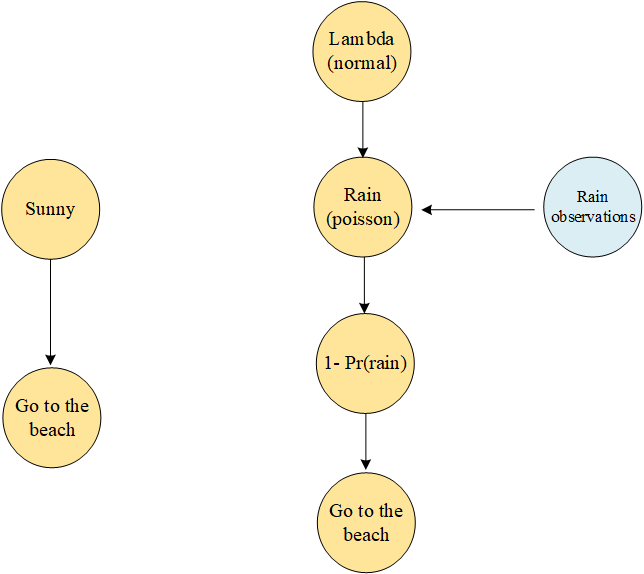
\includegraphics[width=0.7\textwidth]{SectionLetsMath/nonLinearMethods_fig/fig_bayesianNetwork.png}
\captionsetup{type=figure}
\caption{Example of a Bayesian network.}
\label{fig_bayesianNetwork}
\end{figure}

We are interested in sampling the posterior, i.e. to measure the probability of going to the beach, given all these parameters. A technique called Montecarlo Markov Chain (MCMC) permits to sample from the posterior, given the connection between all the random variables of a Bayesian network, and given observations of some of these variables. For example, we have past observations of the probability of rain, from the weather forecasts. MCMC can fit these empirical observations to the Poisson probability distribution and compute all the other parameters of the network consequently.

\section{Analogisers’ methods}
Analogisers proceeds by labelling items depending on their similarity to a set of given items. The simplest approach is the $k$-nearest neighbour, an algorithm computing the distance of a new observation from all the given observations and assigning to it the label of the closes. The formal language of analogisers is the weighting of a specific instance as in the Support Vector Machine whose evaluation metric is the margin. Their search method is the constrained optimization that moves within the boundaries, looking for the best values.\footnote{The package logproj provides methods to deal with analogisers' methods \href{https://github.com/aletuf93/logproj/blob/master/logproj/M_learningMethod/analogizers_models.py}{here}.}

\subsection{Support vector machines}
Support vector machines (SVM) are based on the concept of support vector classifier (SVC); they can be interpreted as a weighted $k$-nearest neighbour. An SVC identifies thresholds are defined to identify regions of the hyperplane containing all the input data. Different regions have different labels. New observations are classified depending on the region of the hyperplane where they fall. The shortest distance between the observation and the threshold dividing the hyperplane’s regions is called margin. \par

By setting thresholds that gives the largest margin, there is a high risk of misclassification if the input dataset contains outliers. For this reason, it is necessary to allow the SVC to misclassify the input data. This way, we have data points falling within a hyperplane’s region with a different label. This is called soft margin classifier or SVC since the observation on the edge of a region, and within the soft margin are called support vectors. The support vectors define the regions’ boundaries. The support vectors always have a $p-1$ dimension, where $p$ is the dimension of the input dataset.\par

A SVC defines hyperplanes $f\left(x\right)=x^T\beta+\beta_0$ such that $y_if\left(x_i\right)>0\ \forall\ i$. The hyperplane which best separates the space is defined by the optimisation problem:

\begin{equation}
\begin{split}
        \max_{\beta,\beta_0,\left|\beta\right|=1}{M}\\
        y_i\left(x_i^T\beta+\beta_0\right)\geq M\ ,\ i=1,\ldots,N\\
\end{split}
\label{eq_svm1}
\end{equation}

In case the classes overlap, it is still possible to maximise M allowing for some points to be on the other side of the margin. Let $\xi$ be a slack variable $\xi={\xi_1,\ldots,\xi_N}$, we have:

\begin{equation}
        y_i\left(x_i^T\beta+\beta_0\right)\geq M-\xi_i
\label{eq_svm2}
\end{equation}
Where the value of $\xi$ indicates a proportional amount by which the prediction is on the wrong side of the margin.\par

SVC have a problem when a region is enclosed by another, i.e. there is no possibility to define a support vector $p$-1 dimensional to separate the two regions correctly. Kernel transformations are used to overcome this problem. The input dataset is projected into a hyperplane with a higher dimension, and then an SVC is used. This procedure is called SVM. Common kernels are polynomial kernel with dimension $d$, that projects the point using a power elevation of their values, or the non-linear radial basis function. 

\section{Connectionists’ methods}
Connectionsts aim at learning by mimic the connection of the human brain. The human brain is composed of interconnected neurons activated by electrical impulses. The formal language of the connectionists is the neural network. A neural network has an input similar to the input from the five senses of a human. Depending on the input, different groups of neurons are activated, producing the output. The evaluation metric of connectionists is a continuous error metric, as the mean squared error (see section \ref{secMSE}) that measures the difference between the know target label, and the output of the neural network. The search algorithm to define the behaviour of the neurons is the gradient descent.\footnote{The package logproj provides methods to deal with connectionists' methods \href{https://github.com/aletuf93/logproj/blob/master/logproj/M_learningMethod/connectionists_models.py}{here}.}

\subsection{Neural Networks}
Neural networks work by mimic a network of neurons. Figure \ref{fig_neuron} illustrate how a mathematical neuron is defined. A neuron has some inputs, a bias input quantity b. All these inputs are summed up and processed by an activation function. This is usually a sigmoid function, as a logistic function, a hyperbolic tangent, a rectified linear (RELU) or a fixed threshold. If the sum of the input is enough to activate the function, a positive output is obtained; otherwise, the energy provided by the inputs is not enough to activate the neuron, that produces a zero.

% INSERT fig_neuron
\begin{figure}[hbt!]
\centering
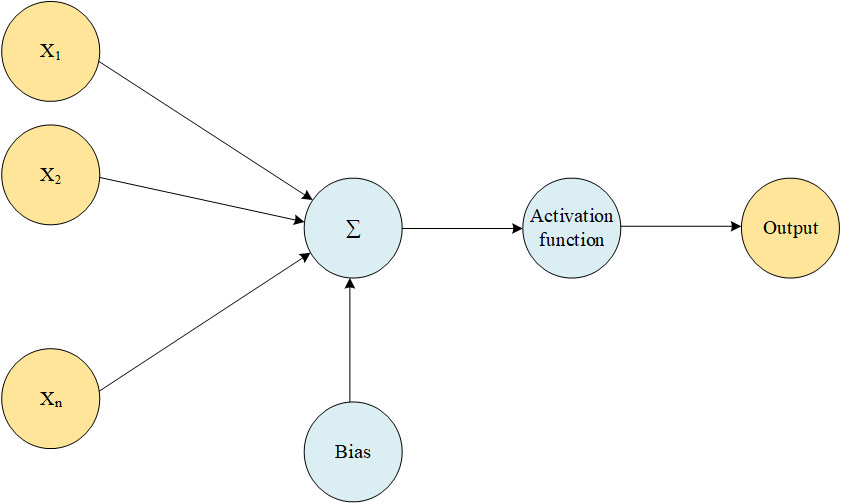
\includegraphics[width=0.7\textwidth]{SectionLetsMath/nonLinearMethods_fig/fig_neuron.png}
\captionsetup{type=figure}
\caption{Schema of a neuron.}
\label{fig_neuron}
\end{figure}

In practice, each neuron works similarly to a logistic regressor. Putting together multiple neurons into deep layers is what they called deep learning. The central idea of a neural network is to extract linear combinations of the input features $X$ to create hidden features $Z$ and model the target as a non-linear function of these features. \par

There are neural networks with complex mechanisms and topologies. For the sake of brevity, we analyse how a single layer neural network works. This model is also known as “single-layer perceptron Let consider the case of classification into $K$ different classes. The model involves:

\begin{itemize}
    \item $p$ input features $x_1,\ldots,x_p$;
    \item $M$ derived features $Z_1,\ldots Z_m,\ldots,Z_M$;
    \item $K$ target $Y_1,\ldots,Y_k,\ldots Y_K$.
\end{itemize}

The main idea is modelling the target $Y$ as a combination of $Z$.

\begin{equation}
        f_k\left(X\right)=g_k(T)
\label{eq_neuralNetwork}
\end{equation}
Where:
\begin{itemize}
    \item $T_k=\beta_0+\beta_k^TZ$, $k=1,\ldots,K$ is a linear combination of the hidden layer features $Z$, with
    \item $Z_m=\sigma(\alpha_{0m}+\alpha_m^TX)$, $m=1,\ldots,M$. 
\end{itemize}

The function $\sigma$ is the activation function, usually the sigmoid function $\sigma\left(v\right)=\frac{1}{1+e^{-v}}$. This function is a non-linear transformation of the input $X$, which is the core of neural networks. If $\sigma$ equals an identity function, all the model collapses to a linear model. $g_k$ is a transformation function to get the final input. For regression the identity function $g_k(T)=T_k$ is used while the softmax function is used for $k$-classification problems $g_k\left(T\right)=\frac{e^{T_k}}{\sum_{l=1}^{K}e^{T_l}}$.\par

Fitting a neural network means to identify the unknown weights $\alpha_{0m},\alpha_m$; $m=1,\ldots,M$ and $\beta_{0m}$; $\beta_k;k=1,\ldots,K$. A neural network use the gradient descent algorithm to find the value of these parameters minimising an error metric as the sum-of-squared errors $\sum_{k=1}^{K}\sum_{i=1}^{N}\left(y_{ik}-f_{k\left(x_i\right)}\right)^2$ for regression, or the cross-entropy  $\sum_{i=1}^{N}\sum_{k=1}^{K}{y_{ik}\log{f_k\left(x_i\right)}}$ for classification.


%\clearpage
\bibliographystyle{ieeetr}
\bibliography{SectionLetsMath/nonLinearMethods_ref.bib}